\chapter{Designing and Implementing the OurPlace Platform}
\label{chap:Design}

Following the engagements covered in Chapter \ref{chap:DesignSpace}, I decided to iterate upon the Park:Learn prototype application. With the aim of creating an application which could be utilised in formal and informal learning contexts, I examined previous mobile learning research (summarised in Chapter \ref{chap:MobileLearning}) to produce a number of design goals for the technology. This application would also aim to follow the implications for design (as described in section \ref{sec:SuggestionsCivicLearning}) derived from the findings of the previous exploratory study. This chapter describes the design goals for the technology, why those goals were chosen, a detailed overview of the application itself and how it evolved over the course of the remainder of the project. Much of the work covered by this chapter was peer-reviewed and published at MobileHCI 2018 \citep{Richardson2018}, with the paper being co-authored by Doctors Pradthana Jarusriboonchai, Kyle Montague and Ahmed Kharrufa. 

\section{Technology Design Goals}

Based on the findings of previous works and the design engagements covered in Chapter \ref{chap:DesignSpace}, we produced several design goals (DGs). This section describes each design goal and the rationale behind choosing them.

% reference like this: (addresses \hyperref[DG1]{DG1})

\subsection*{ DG1: Utilize local places and communities as learning resources }
\phantomsection
\label{DG1}

This first goal is that the final technology should support greater utilisation of local places (e.g. parks, buildings, towns, rooms, etc) and the communities which surround, inhabit and have built relationships with them as learning resources. This primarily relates to the previously discussed Park:Learn studies, during which we found that places' stakeholders can offer not only a diverse knowledge base, but also a large variety of motivations, aspirations and tensions related to place. We suggested that mobile learning technologies might be able to make use of these social infrastructures, by giving places’ stakeholders a platform for sharing their values through designing and sharing learning activities in authentic contexts \citep{Richardson2017}. This would not only support learners in situating their learning activities within authentic physical environments, but might also introduce them to new communities of practice which they may enter and develop an expertise through interactions with them \citep{lave1991situated}.

\subsection*{ DG2: Support seamless outdoor and classroom use }
\phantomsection
\label{DG2}

As noted by Sharples, mobile learning does not necessarily always take place in one context, or even one fixed level of formality \citep{Sharples2013}. He presents mobile learning as taking place on a linear spectrum: from formal, classroom and curriculum-based learning activities, to ones are informal, creative and \textit{mobile} \ref{fig:learningContextDimension}. However, while these contexts are different, they can still be connected---Kuh argues that learning experiences across contexts can be bound into a `seamless learning' narrative \citep{Kuh1996}. In order to support this seamless use across contexts, our design should encompass as many of Wong and Looi's `desirable dimensions' of seamless learning as possible \citep{Wong2011} (all ten dimensions are listed in section \ref{sec:Seamless}). Multiple examples of seamless mobile learning applications which adhere to some (or all) of these dimensions already exist. For example, Zydeco supports the use of multiple types of devices across multiple locations (classrooms and museums), utilising both digital and physical learning resources \citep{kuhn2011}.

\subsection*{ DG3: Support a variety of pedagogical approaches and stakeholder requirements }
\phantomsection
\label{DG3}

The final `desirable dimension' listed by Wong and Looi is that seamless mobile learning technologies should encompass multiple pedagogical models, as a diversity of learning experiences requires the deployment of different learning models \citep{Wong2011}. For example, the learning theory of constructionism and project-based learning pedagogies (as covered in section \ref{sec:ConstructionismPBL}) have different requirements to more traditional classroom teaching methods. Sessions within these pedagogies will often have different goals, with the intended outcomes also changing according to the stakeholders' agenda (e.g. teachers may want to be able to provide evidence of students' learning, while park rangers and volunteers may want to promote place-making in an attempt to nurture stewardship and volunteerism \citep{Richardson2017}). As such, our technology needs to be flexible enough to support different goals, learning processes and intended outcomes, ideally without relying heavily on additional tools.

\subsection*{ DG4: Support a wide range of user ages and technical expertise }
\phantomsection
\label{DG4}

While it has almost become a truism that children are frequently technologically adept, care still needs to be taken to support age and ability groups who may struggle with reading or typing large quantities of text (as shown to be an issue in MyArtSpace \citep{Vavoula2009} and deliberately avoided in Zydeco \citep{kuhn2011}). Furthermore, engaging with a large variety of place stakeholders means that older age groups---who may not be as technologically literate---may wish to use the technology. Our technology design will therefore strive to minimise (or provide alternatives to) large amounts of typing, and, as suggested by Land, attempt to support a range of learner ages and reading abilities through the use of simple, varied but semantically consistent visual interfaces \citep{Land2015}.

\subsection*{ DG5: Support learning and reflection in authentic learning contexts }
\phantomsection
\label{DG5}

Our observations in the initial engagements (as well elements found in prior work, such as in Mobilogue \citep{Giemza2013}) demonstrated that giving students greater control and opportunities for creativity can act as a motivating factor. As such, our design aimed to utilise interaction methods on mobile devices which support student creativity and control in authentic learning environments. That said, while not all mobile learning projects made use of the learner's context as a learning environment or resource \citep{Frohberg2009}, even fewer promote learner reflection within the authentic learning environment. For example, MyArtSpace \citep{Vavoula2009} and Sense-It \citep{Sharples2017} encourage learners to use the technology to collect data or take brief notes and observations, rather than engage in in-depth reflection in-situ. This is certainly useful, and should have a place in the final design. However, we wanted our design to also support immediate reflection from the learner, without the need to return to the classroom. This level of immediacy should also apply to activity creation and data collection, in an attempt to minimise the learner being distracted from authentic engagement with the learning context. 

\subsection*{ DG6: Support mobile learning in resource-limited schools }
\phantomsection
\label{DG6}

As discussed in sections \ref{sec:DigitalCivics} and \ref{sec:ParkContext}, the UK as a whole is enduring an extended period of austerity and local authorities have had to cut funding wherever possible. As a result, many schools have become resource-limited and may struggle to justify spending money on having more smart mobile devices for classroom use, despite them becoming more affordable and fashionable within education. While our final software design will require the use of a smartphone or tablet, it must take steps to minimise the financial strain placed upon schools in its use. The design should: require minimal teacher time to set up and use, as well as access and download student work; support the sharing of devices between multiple students, either through group work or the ability to save and clear progress to allow another student to start activities afresh (as seen in Mobilogue \citep{Giemza2013}); and support the offline caching of data, allowing teachers to pre-load content in the classroom prior to trips, or queuing student work for later upload (avoiding expensive 4G mobile data contracts).

\section{An Overview of ParkLearn and OurPlace}

ParkLearn, the prototype application discussed in Chapter \ref{chap:DesignSpace}, was further developed to meet these design goals. While the early version was created as a simple proof of concept and acted as a technology probe, later versions featured far greater functionality. This section will detail the application: its features, its implementation, and how it evolved over time into the later OurPlace app. As the two versions are extremely similar, for the sake of clarity `OurPlace' will be used as the application's name for the rest of this chapter. Significant differences in the two applications' features or implementations will be noted explicitly.

\subsection{The Anatomy of an Activity}
\label{sec:ActivityOverview}
Core to the OurPlace application is the concept of `Activities'. In terms of user interaction, they are the more or less the same as the ones introduced in the prototype ParkLearn application, based on the original jigsaw workshop activity (Figure \ref{fig:rangerJigsaw}). While the Activities in the prototype version were hard-coded into the application, later versions allowed users to create their own Activities, or complete other people's. They are delivered to the mobile app by the remote server in the standard JSON data format (see section \ref{sec:ImplementationWeb}), allowing for the app to allow users to discover and open Activities in numerous ways (see section \ref{sec:SharingActivities}).

Activities are typically based on a particular topic, location or subject (e.g. `\textit{Exploring the Rose Garden}'). Each OurPlace Activity must feature a title and a short (up to 150 characters) description, which gives the learner some insight into what the Activity will be about (Figure \ref{fig:ActivityExample}). Additionally, Activity creators may choose to include an image to represent the Activity: this will appear on the application's feeds, and at the top of the main Activity screen. The application supports taking this image directly through the device's camera, or the use of pre-existing images from the user's photo gallery (allowing users to select images they prepared earlier, or downloaded from the Internet). By allowing both options, activity creators are able to either create their Activities within the relevant physical context (addresses \hyperref[DG5]{DG5}) or remotely, which may be easier if preparing for a future school trip (addresses \hyperref[DG6]{DG6}).

\begin{figure*}
  \centering
  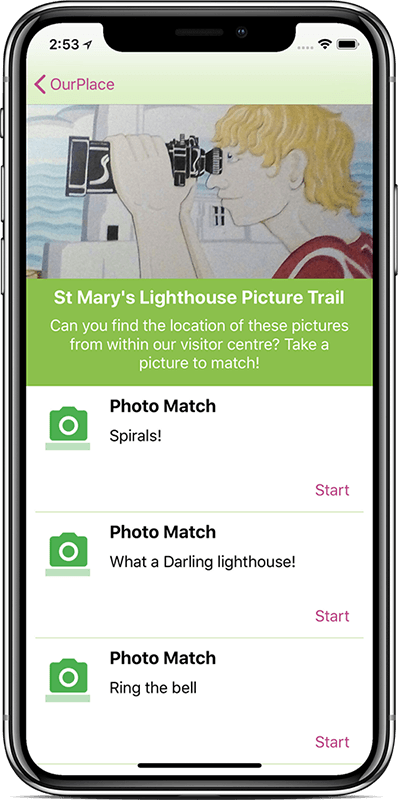
\includegraphics[width=0.85\columnwidth]{images/chapter05/activity.png}
  \caption{ A simple Activity in the OurPlace iPhone app. The Activity's image, title and description appear at the top, with Tasks underneath. The Task Type of each Task is made known to the user by displaying its name and icon. The screen can scroll vertically if there are more Tasks than can be displayed at once. }~\label{fig:ActivityExample}
\end{figure*}

Each Activity must also feature at least one `Task'. Tasks are modular, and each one centres around a single user interaction (e.g. `\textit{Take a Photo}'). A large number of variations (`Task Types') of Tasks are available, supporting a berth of different interactions (addresses \hyperref[DG3]{DG3}). Table \ref{tab:TaskTypes} shows all of the different Task Types available in OurPlace (note that `\textit{Scan the QR Code}' was introduced in OurPlace, and was not available in ParkLearn). An Activity can have an unlimited number of Tasks, and the learner is able to complete them in any order.

\begin{table}
  \centering
  \begin{tabular}{l|p{110mm}}
    % \toprule
    {\small\textit{Task Type}}
    & {\small \textit{Interaction Description}} \\
    \midrule
    \small Information & \small Read some written information, with an optional accompanying image and hyperlink \\
    \small Listen to Audio & \small Listen to a given audio recording \\
    \small Take a Photo & \small Use the camera to take still images \\
    \small Photo Match & \small Use the camera to match an existing photo given as an overlay \\
    \small Draw a Picture & \small Draw a picture onto a blank canvas \\
    \small Draw on Photo & \small Draw on top of a given image \\
    \small Record Video & \small Record a video using the camera \\
    \small Record Audio & \small Record audio using the device's microphone \\
    \small Map Marking & \small Mark a given number of locations onto a Google Map \\
    \small Location Hunt & \small Track down a target location by observing your reported distance \\
    \small Scan the QR Code & \small Find and scan the correct QR code \\
    \small Multiple Choice & \small Choose a response from text options \\
    \small Text Entry & \small Enter a response using the keyboard
    % \bottomrule
  \end{tabular}
  \caption{The Task Types available in the OurPlace application}~\label{tab:TaskTypes}
\end{table}

As noted in Chapter \ref{chap:DesignSpace}, each of these interactions were chosen either because they put an element of creative control into the hands of the learner (\textit{Take a Photo, Draw a Picture, Draw on Photo, Record Video, Record Audio}) (addresses \hyperref[DG5]{DG5}), took advantage of the devices’ hardware capabilities across different contexts (\textit{Listen to Audio, Map Marking, Location Hunt, Scan the QR Code}) (addresses \hyperref[DG2]{DG2}), emulated features of the learning materials already in use by teachers and park rangers (\textit{Information, Multiple Choice, Text Entry}) (addresses \hyperref[DG3]{DG3}), or a combination of all of the above.

The OurPlace app also features the concept of `Follow-Up Tasks', which were not available in ParkLearn. Follow-Up Tasks act as children to a chosen parent Task, only becoming available when the parent has been completed. For example, a Task might ask the learner to take a picture of the item in a museum they found most interesting, and then a Follow-Up Task could ask them to record an audio clip of them explaining what was interesting about it. Having this ability allows Activity designers to encourage students to reflect through the application, while still in the authentic learning environment (addresses \hyperref[DG5]{DG5}).

\subsection{Creating Activities}

\begin{figure*}
  \centering
  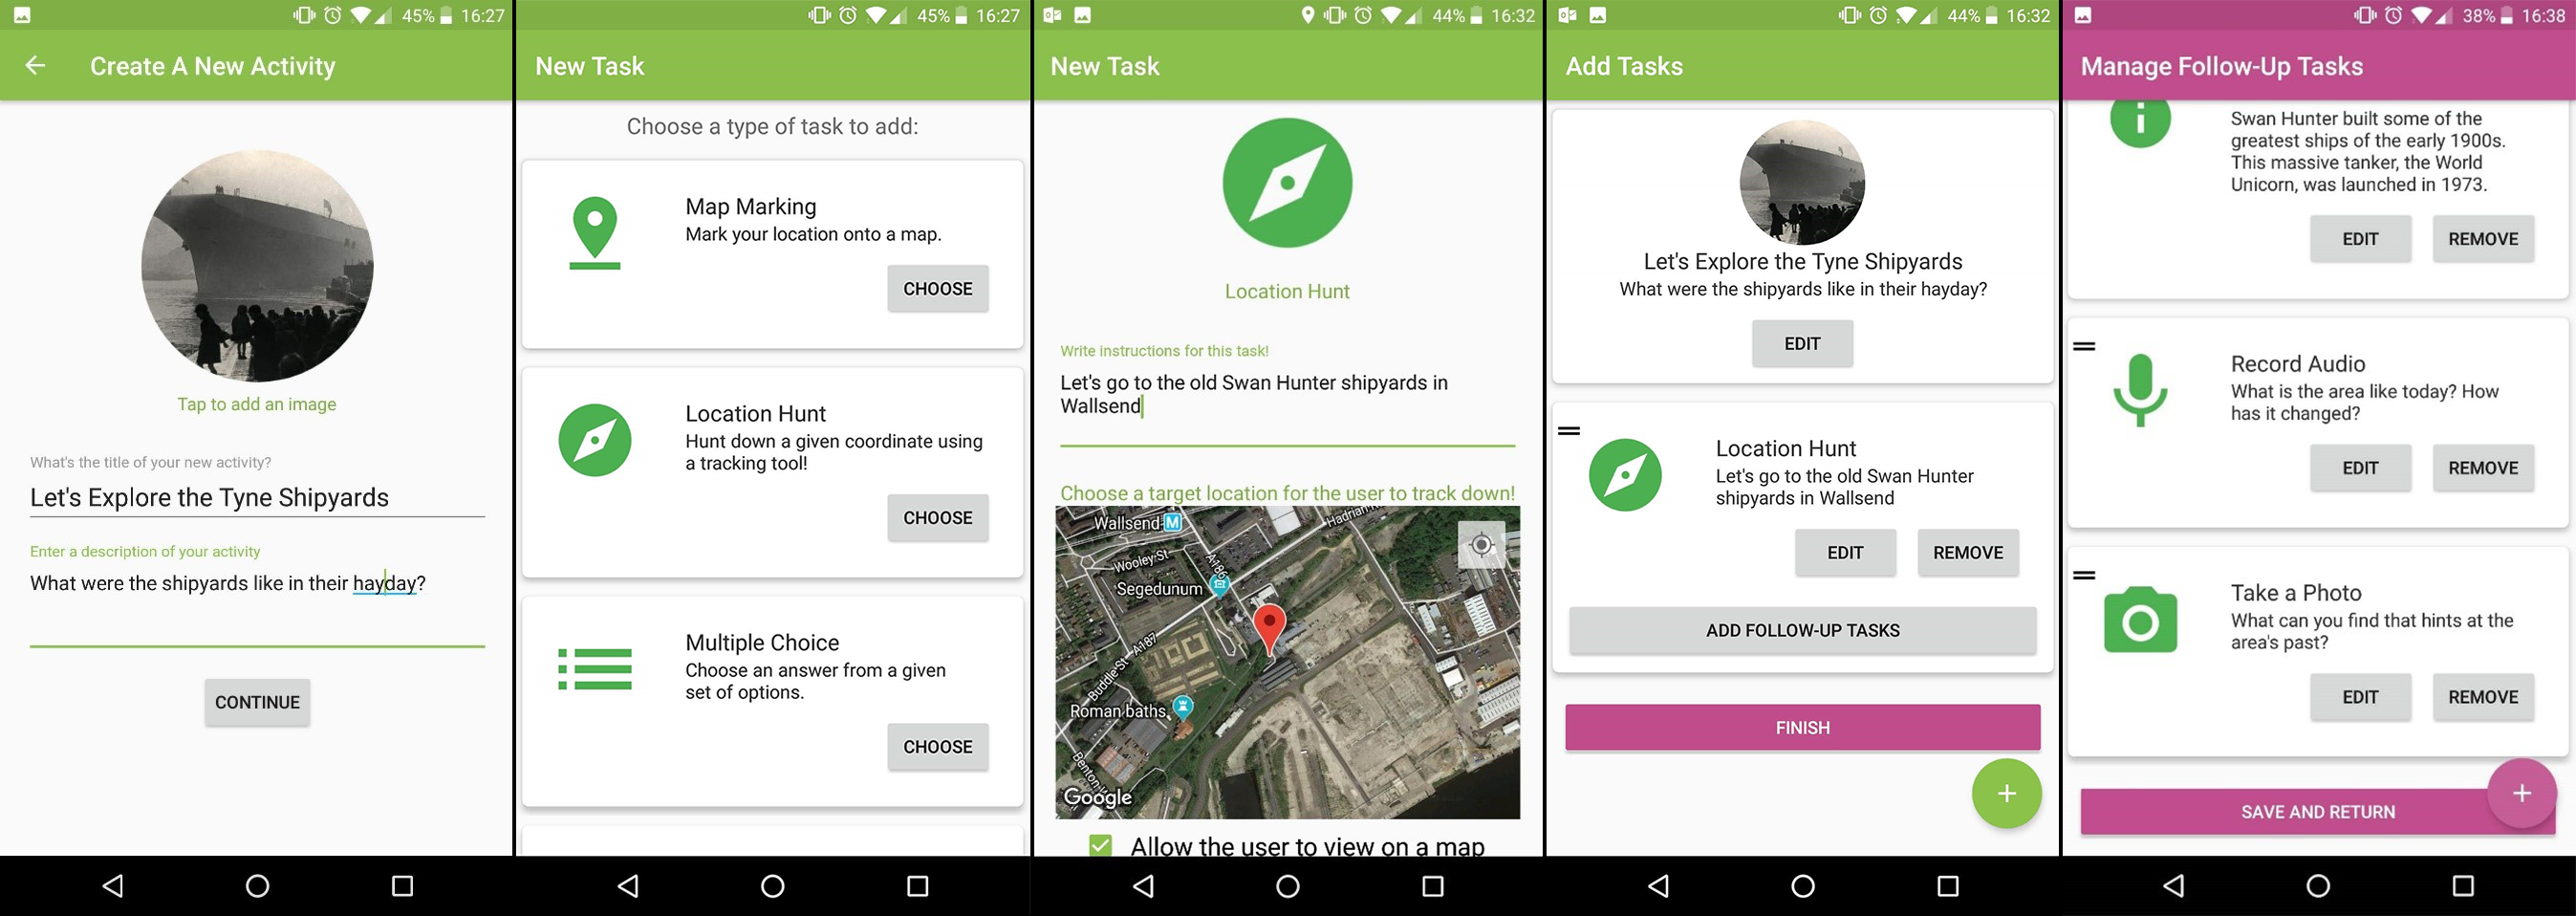
\includegraphics[width=1\columnwidth]{images/chapter05/activityCreation}
  \caption{Creating an OurPlace activity (left to right): a) Choosing the activity's title, description and image; b) Choosing a Task Type to add; c) Adding a \textit{Location Hunt} Task, with description and target coordinates; d) The new Task in the Activity; e) Adding Follow-Up Tasks to the \textit{Location Hunt}  }~\label{fig:ActivityCreation}
\end{figure*}

\subsection{Sharing, Discovering and Launching Activities}
\label{sec:SharingActivities}

\subsubsection{The Highlights Feed and Location}

\subsubsection{Share Codes and QR Codes}

\subsection{Completing Activities}

\section{Implementation of the OurPlace Mobile Applications}
\label{sec:ImplementationMobile}

\subsection{Improvements over ParkLearn}

\subsubsection{Developing the iOS Application}

\subsubsection{Adding Follow-Up Tasks}

\subsubsection{QR Code Task Types}

\subsubsection{Other General Improvements}


\subsection{The OurPlace App}

OurPlace is the current iteration of the open-source ParkLearn platform, with an expanded feature set and re-branded to support its use in contexts outside of local parks \citep{Richardson2018a}. Consisting of a website and mobile applications for both Android and iOS, OurPlace supports the creation of--and sharing and engagement with--m-learning activities (`Activities'), each of which is built up from smaller, modular tasks (`Tasks'). These tasks each consist of a specific interaction (`Task Type'), which either promote creativity, emulate traditional classroom learning materials or use the device's hardware to give context-specific experiences (Table~\ref{tab:TaskTypes}). With the exception of \textit{Scan the QR Code}, all of these Task Types were present in the original ParkLearn application. OurPlace also adds support for `Follow-Up Tasks', which allow activity creators to add sub-tasks which unlock once their parent task has been completed (Figure~\ref{fig:ActivityCreation}.e). This supports the design of more complicated combinations of interactions (for example: a \textit{Location Hunt} could unlock a \textit{Record Audio} and \textit{Take a Photo} once the user arrives at a designated location).


Activities are created within the app itself. After supplying a title, description and an optional image (Figure~\ref{fig:ActivityCreation}.a), the designer creates the Tasks that make up the Activity (Figure~\ref{fig:ActivityCreation}.b). Each Task Type requires at least a written instruction for the learner (e.g. A \textit{Location Hunt} might say \textit{`Can you find Carter's Well?'}), but some of them require some additional customization (e.g. supplying geographic coordinates by tapping on a Google Maps view) (Figure~\ref{fig:ActivityCreation}.c). No additional equipment or software is required to create activities (other than \textit{Scan the QR Code}, which requires creators to print the generated QR code from the OurPlace website). Uploaded activities can be edited for testing, feedback and iteration--allowing for the `essential elements' of reflection, critique and revision of a final public product \citep{Larmer2015}. 

\section{Implementation of the API and Website}
\label{sec:ImplementationWeb}

\section{Development of the Technology}

\subsection{Why use the Xamarin framework?}
The OurPlace platform is a system consisting of smartphone applications for the
Android and iOS (Apple iPhone and iPad) operating systems, a website and an
online application programming interface (API). It was decided that in order to
support as many schools, groups and individuals as possible, both of the main
smartphone OSs should be supported (Android and iOS). Furthermore, in order to
provide a high quality experience which conformed to each platform's expected
design metaphors,  supported access to all of the devices' hardware features and
didn't require a constant internet connection, I decided to produce `native'
applications for each platform (that is, rather than produce something like a
website which would be the same across all platforms). Ordinarily, this would
result in having to produce software in multiple programming languages: for
example, Android applications are usually written in either Java or Kotlin,
whereas iPhone apps are written in Objective-C, which is very different. As the
project was mostly a one-man show, dedicating large amounts of time to learning,
developing, iterating and maintaining systems across multiple languages was
unrealistic. 

In the end, the decision was made to develop the mobile applications using the
Xamarin framework. This framework takes code written in C\# and compiles it into
`native' applications, meaning that apps look, feel and act like software
written in the different platforms' specific languages. This gave the advantage
of sharing the same programming language across both applications, without
losing out on any major features and allowing for common code (functionality
identical across the two applications, e.g. making requests to the server) to be
shared across the projects. To fully capitalise on this code sharing advantage,
it was decided to take this further and produce the website and API in C\#. As a
result, every component of the OurPlace platform can be opened within the same
Visual Studio `solution', significantly speeding up the development process.

\subsection{Disadvantages to using Xamarin}
While developing the mobile applications with the Xamarin framework
significantly reduced to upfront time investment in the development process, it
certainly had its trade-offs which became more apparent as the project grew.
Having all of the OurPlace code available within one solution (discussed in
\ref{sec:OurPlaceSolution}) was certainly convenient and minimised code
duplication, but when combined with Xamarin's more demanding build process it
created large performance overheads. This, combined with issues of documentation
being in other programming languages (particularly on the iOS application),
impeded the development workflow, frequently slowing it to a crawl. At the end
of the project, it is difficult to say if significant time was saved by using
Xamarin over the two platforms' `native' development tools. However, anyone
considering these options should note that recent developments to Visual Studio
and the Xamarin framework have significantly improved performance, which may somewhat
mitigate these issues.

\subsection{A Brief Tour of the OurPlace Visual Studio Solution}
\label{sec:OurPlaceSolution}
All of the OurPlace code is open source, and can be viewed at
\url{https://github.com/GSDan/OurPlace}. Using C\# and Microsoft's .NET Framework
across the OurPlace platform afforded it being accessible within a single Visual
Studio solution, split into four smaller component projects:
\textit{OurPlace.Common}, \textit{OurPlace.API}, \textit{OurPlace.Android} and
\textit{OurPlace.iOS}.

\paragraph{OurPlace.Common}
This is a .NET Standard 2.0 project, which acts as a `library' of functions and
serves the other projects within the solution. It contains shared data models,
interfaces and common core functionality, including managing the apps' local
files, authenticating with the server, polling it for the latest OurPlace
activities and uploading new activities and responses. This is the only project
which is referenced from elsewhere in the solution.

\paragraph{OurPlace.API}
This project uses version 4.6.1 of the .NET Framework, and contains an ASP .NET
website, a Web API 2 powered API and a Code First, Entity Framework database.
This project is discussed in detail in section \ref{sec:ImplementationWeb}.

\paragraph{OurPlace.Android}
This project contains all of the code specific to the Android application.
Written in C\# using the Xamarin.Android framework, a `native' Android application is
produced upon compilation, supporting devices running Android versions as old as
4.1 (Jelly Bean, 2012) and targeting the latest features found in version 8.1
(Oreo, 2017). This project is discussed in detail in section
\ref{sec:ImplementationMobile}.

\paragraph{OurPlace.iOS}
This project contains all of the code specific to the iPhone/iPad application.
Written in C\# using the Xamarin.iOS framework, a `native' iOS application is
produced upon compilation. The application requires a minimum of iOS 10, which
is supported by devices as old as the iPhone 5 (released 2012). This project is
discussed in detail in section \ref{sec:ImplementationMobile}.